\documentclass[12pt,a4paper]{report}

\usepackage[T2A]{fontenc}
\usepackage[utf8]{inputenc}
\usepackage[english,russian]{babel}
\usepackage{amsmath}
\usepackage{amsfonts}
\usepackage{amssymb}
\usepackage{graphicx}
\usepackage{listings}

\voffset -24.5mm
\hoffset -5mm
\textwidth 173mm
\textheight 240mm
\oddsidemargin=0mm \evensidemargin=0mm

\lstdefinestyle{CppCodeStyle}{
	basicstyle=\footnotesize\ttfamily,
	language={[ANSI]C++},
	keywordstyle=\bfseries,
	showstringspaces=false,
	morekeywords={include, printf},
	commentstyle={},
	texcl=true,
	frame=single,
	breaklines=true,
	extendedchars=\true
}

\begin{document}
	\begin{titlepage}
\begin{center}

\textbf{Санкт-Петербургский политехнический университет Петра Великого}

\vspace{5mm}
Институт компьютерных наук и технологий

\vspace{5mm}
Кафедра компьютерных систем и программных технологий

\vspace*{\fill}

\huge{ОТЧЕТ}

\Large{о лабораторной работе №1}

\large{по дисциплине: <<Параллельные вычисления>>}

\vspace*{2mm}
\large{Тема работы: <<Подсчет количества русских слов в тексте>>}

\vspace*{\fill}
\end{center}

%\begin{flushright}
\begin{large}
\hspace{0.4\linewidth} \textbf{Работу выполнил студент}

\vspace{5mm}
\hspace{0.4\linewidth} 53051/3 \hspace{1cm} \textit{Скрипаль Б.А.}

\vspace{3mm}
\hspace{0.4\linewidth} \textbf{Преподаватель}

\vspace{5mm}
\hspace{0.4\linewidth} \underline{\hspace{2cm} } \hspace{3mm} \textit{Стручков И.В.}
\end{large}
%\end{flushright}

\vspace*{3cm}

\begin{center}
\normalsize Санкт-Петербург\\2016
\end{center}
\end{titlepage}
	
	\renewcommand{\thesection}{\arabic{section}}
	\tableofcontents
	\pagebreak
	
	\setcounter{totalnumber}{10}
	\setcounter{topnumber}{10}
	\setcounter{bottomnumber}{10}
	\renewcommand{\topfraction}{1}
	\renewcommand{\textfraction}{0}
	
	\section{Постановка задачи}
		Реализовать программу, подсчитывающую количество русских слов в тексте при помощи трех технологий:
		\begin{enumerate}
			\item Последовательная реализация;
			\item Параллельная реализация при помощи POSIX threads;
			\item Параллельная реализация при помощи технологии MPI.
		\end{enumerate}
		Сравнить времена выполнения программ, в зависимости от окружения, а так же от количества потоков (процессов) для вариантов 2 и 3.
	\section{Реализация}
		\subsection{Последовательное выполнение}
			В качестве параметров программе передается имя файла с текстом. После 
			чего программа выдает результат в следующем формате: в первой строке 
			вывода будет записано время выполнения программы в миллисекундах, после 
			чего выводится количество повторений слов в формате \textit{"Слово 
			Количество\_повторений"}.
				
			Программа работает по следующему алгоритму:
			\begin{enumerate}
				\item Анализ входных параметров для получения имени файла.
				\item Инициализируем глобальный вектор для хранения слов и map для 
				хранения повторений слов.
				\item Считываем входной файл в массив типа char.
				\item Инициализируем таймер и получаем время начала работы программы.
				\item Последовательно берем каждое новое слово в строке, до тех пор, 
				пока не закончится строка и:
					\begin{itemize}
						\item Если слово не находится в векторе встреченных слов, то 
						добавляем его в вектор и добавляем в map пару типа 
						\textit{Новое\_слово 1}.
						\item Если слово находится в векторе, то увеличиваем 
						соответствующее значение в map на 1.
					\end{itemize}
				\item Считываем время завершения работы и находим время выполнения.
				\item Выводим время выполнения, а так же содержимое map и вектора.
			\end{enumerate}
				
			Исходный код программы приведены в листинге 1.
				
		\subsection{Выполнение при помощи pthreads}
				В качестве параметров программе передается количество потоков и имя 
				файла с текстом. После чего программа выдает результат в следующем 
				формате: в первой строке вывода будет записано время выполнения 
				программы в миллисекундах, после чего выводится количество повторений 
				слов в формате \textit{"Слово Количество\_повторений"}.
					
				Программа работает по следующему алгоритму:
				\begin{enumerate}
					\item Анализ входных параметров для получения имени файла и 
					количество потоков.
						\item Инициализируем глобальный вектор для хранения слов и map для хранения повторений слов, а так же мьютекс для обеспечения совместного доступа к глобальным переменным.
						\item Считываем входной файл в массив типа char.
						\item Инициализируем таймер и получаем время начала работы программы.
						\item Разбиваем входной массив на n (n - количество потоков), массивов примерно одинаковой длинны. Для этого входную строку делим на n равных частей, после чего смещаем каждую границу до первого разделяющего символа (пробела, точки, запятой и т.д.).
						\item Для каждого из потоков запускаем функцию подсчета количества слов и переводим его в отсоединенный режим:
						\begin{enumerate}
							\item Инициализируем локальные вектор и карту для подсчета слов.
							\item Последовательно берем каждое новое слово в строке, до тех пор, пока не закончится строка и:
							\begin{itemize}
								\item Если слово не находится в векторе встреченных слов, то добавляем его в вектор и добавляем в map пару типа \textit{Новое\_слово 1}.
								\item Если слово находится в векторе, то увеличиваем соответствующее значение в map на 1.
							\end{itemize}
							\item Переводим мьютекс в заблокированное состояние.
							\item Объединяем локальные вектор и карту с глобальными вектором и картой.
							\item Разблокируем мьютекс.
						\end{enumerate}
						\item Ожидаем завершения всех потоков.
						\item Считываем время завершения работы и находим время выполнения.
						\item Выводим время выполнения, а так же содержимое map и вектора.
					\end{enumerate}
				
				Исходный код программы представлен в листинге 3.
				
			\subsection{Выполнение при помощи mpi}
					В качестве параметров программе передается количество процессов и имя файла с текстом. После чего программа выдает результат в следующем формате: в первой строке вывода будет записано время выполнения программы в миллисекундах, после чего выводится количество повторений слов в формате \textit{"Слово Количество\_повторений"}.
					
					Программа работает по следующему алгоритму:
					\begin{enumerate}
						\item Анализ входных параметров для получения имени файла и количества процессов.
						\item Инициализируем глобальный вектор для хранения слов и map для хранения повторений слов.
						\item Считываем входной файл в массив типа char.
						\item Инициализируем таймер и получаем время начала работы программы.
						\item При помощи функции \textit{MPI\_Init} разбиваем процесс на несколько процессов. При этом процесс с ID 0 будет "мастером", а остальные процессы будут "служебными". После чего для каждого из типов процессов будет свой алгоритм выполнения.
						\item Процесс-мастер:
							\begin{enumerate}
								\item Разбиваем входную строку на n (n - количество служебных процессов) по такому же принципу, как в многопоточной программе.
								\item Передаем каждому из служебных процессов последовательно два сообщения:
									\begin{itemize}
										\item Размер строки, которую собираемся передать.
										\item Подстроку, которую будет обрабатывать этот служебный процесс.
									\end{itemize}
								\item Получаем от каждого из служебного процесса последовательно следующие сообщения:
									\begin{itemize}
										\item Размер строки, которую собираемся передать.
										\item Подстроку с результатом подсчета слов формата \textit{Слово Количество\_повторений}.
									\end{itemize}
								\item Разбираем строку и обновляем глобальные вектор и карту по аналогии с последовательной программой.
								\item Выводим время завершения обработки.
								\item Выводим результаты.
							\end{enumerate}
						\item Служебный процесс:
							\begin{enumerate}
								\item Получаем от процесса мастера сообщение с длинной строки, которую необходимо принять и инициализируем память по эту строку.
								\item Получаем строку с текстом.
								\item Инициализируем локальные вектор и карту для подсчета слов.
								\item Последовательно берем каждое новое слово в строке, до тех пор, пока не закончится строка и:
									\begin{itemize}
										\item Если слово не находится в векторе встреченных слов, то добавляем его в вектор и добавляем в map пару типа \textit{Новое\_слово 1}.
										\item Если слово находится в векторе, то увеличиваем соответствующее значение в map на 1.
									\end{itemize}
								\item Превращаем вектор и карту в строку вида \textit{"Слово Количество\_повторений"}.
								\item Отправляем процессу-мастеру сообщение с длинной полученной строки.
								\item Отправляем процессу-мастеру сообщение с созданной строкой.
							\end{enumerate}
					\end{enumerate}
				
				Исходный код параллельной программы приведены в листинге 2.
				
		\section{Тестирование производительности программ}
			\subsection{Программа тестирования}
				Для автоматизации тестирования производительности было решено написать 
				следующий скрипт (листинг 4).
				
				Скрипт работает по следующему алгоритму:
				\begin{enumerate}
					\item Очищаем прошлые результаты.
					\item Подготавливаем директории для результатов теста.
					\item Выполняем сборку задач.
					\item Для каждого из тестовых файлов выполняем:
						\begin{enumerate}
							\item Запускаем последовательную программу и записываем результат выполнения в файл \textit{Тестовая\_директория/Имя\_файла.result.serial}.
							\item Запускаем параллельную программу с 4 потоками и записываем результат выполнения в файл \textit{Тестовая\_директория/Имя\_файла.result.thread}.
							\item Для проверки корректности работы программы находим разницу между результатами выполнения между последовательной и параллельной и последовательной и mpi программами и выводим их в файлы \textit{Тестовая\_директория/ Имя\_файла. diff .serial .thread} и \textit{Тестовая\_директория/ Имя\_файла .diff .serial .mpi} соответственно.
						\end{enumerate}
					\item Запускаем последовательную программу 50 раз для сбора статистики времени работы и записываем результаты работы в файл \textit{Тестовая\_директория/ result .serial .repeate}.
					\item Запускаем параллельную программу для 1, 2, 4 потоков 50 раз для сбора статистики времени работы и записываем результаты работы в файл \textit{Тестовая\_директория/ result . threads. Количество\_потоков .repeate}.
					\item Запускаем параллельную средствами mpi программу для 2, 3, 4 потоков 50 раз для сбора статистики времени работы и записываем результаты работы в файл \textit{Тестовая\_директория/ result . threads. Количество\_процессов .repeate}.
				\end{enumerate}
			\subsection{Результаты тестирования}
				Тестирование производилось на компьютере со следующими характеристиками:
				
				\begin{itemize}
					\item Процессор Intel Core i5 4690 (Haswell)
						\begin{itemize}
							\item 4 физических ядра;
							\item 4 потока;
							\item Тактовая частота 3.5 ГГц.
						\end{itemize}
					\item Двуканальная память DDR3, размером 8 Гб;
					\item Установленная ОС - Ubuntu 15.10 (версия ядра 4.2).
				\end{itemize}
				В качестве тестируемого файла был выбран файл большого размера (около 
				17Мб) для того, что бы основное время выполнения приходилось на подсчет 
				количества слов. Результаты тестирования приведены в 				
				таблице~\ref{tab:totalTab}.
				\begin{table}[h]
					\caption{\label{tab:totalTab} Результаты работы программ.}
					\begin{center}
						\begin{tabular}{|c|c|c|c|}
							\hline
							\textbf{Тип программы} & \textbf{Мат. ожидание} & \textbf{СKO} & \textbf{Дов. интервал}\\
							\hline
							Последовательная & 2253,34 & 25,48 & 7,06\\
							\hline
							pthreads 1 поток & 2295,96 & 20,18 & 5,59\\
							\hline
							pthreads 2 потока & 1195,1 & 12,41 & 3,44\\
							\hline
							pthreads 4 потока & 651,76 & 7,14 & 1,98\\
							\hline
							pthreads 8 потоков & 643,8 & 10,11 & 2,96\\
							\hline
							pthreads 16 потоков & 619,22 & 13,71 & 3,8\\
							\hline
							mpi 1 служебный процесс & 2272,9 & 7,38 & 2,04\\
							\hline
							mpi 2 служебных процесса & 1190,96 & 6,71 & 1,86\\
							\hline
							mpi 3 служебных процесса & 835,58 & 5,03 & 1,40\\
							\hline
							mpi 4 служебных процесса & 963,52 & 82,84 & 22,96\\
							\hline
							mpi 8 служебных процессов & 1342,82 & 190,79 & 52,89\\
							\hline
							mpi 16 служебных процессов & 2496,78 & 216,54 & 60,20\\
							\hline
						\end{tabular}
					\end{center}
				\end{table}
				
				Как видно из результатов программы, при задании минимального количества 
				потоков (1) для второй программы и минимального количества процессов 
				для третьей (2), время выполнения отличается не сильно. Графическое 
				отображение зависимости времени выполнения для второй программы 
				представлены на рисунке~\ref{ris:threads} и для третьей на 
				рисунке~\ref{ris:mpi}.
				\begin{figure}[h]
					\center{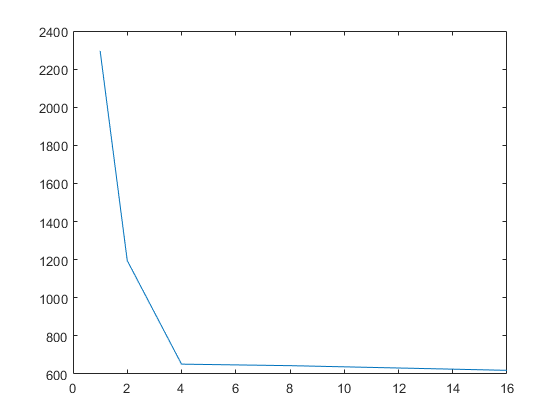
\includegraphics[width=0.7\linewidth]{res/threads}}
					\caption{Зависимость времени выполнения от количества потоков.}
					\label{ris:threads}
				\end{figure}
				
				\begin{figure}[h]
					\center{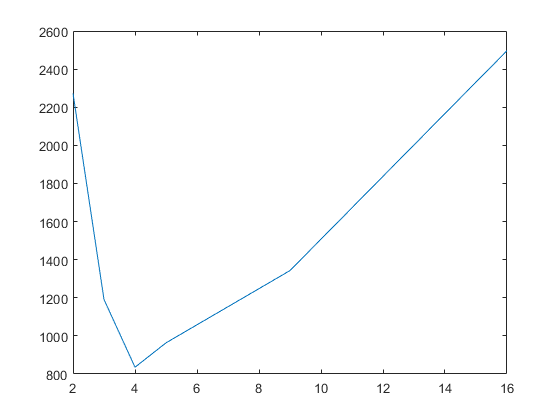
\includegraphics[width=0.7\linewidth]{res/mpi}}
					\caption{Зависимость времени выполнения от количества процессов.}
					\label{ris:mpi}
				\end{figure}
				
				Как видно из результатов работы, при увеличении числа процессов 
				(потоков) до количества ядер позволяет значительно уменьшить время 
				выполнения программы (до 3.5 раз), после чего две программы ведут себя 
				несколько по разному. Вторая программа (в которой используются потоки) 
				при задании количества потоков больше, чем количество ядер процессора 
				практически не ухудшает свои временные показатели 
				(рисунок~\ref{ris:threads}). Программа, в которой использовалась 
				технология MPI (рисунок~\ref{ris:mpi}), напротив, при задании 
				количества процессов, больше, чем колличество ядер значительно ухудшила 
				свои показатели. Это, скорее всего, связано с процедурой планирования в 
				ОС Ubuntu: так как в ней производится планирование на уровне процессов, 
				при создании большого количества процессов, каждый из которых сильно 
				загружает ЦП, необходимо частое переключение контекстов, что 
				значительно замедляет работу.
			
			\section{Вывод}
			
				Целью данной лабораторной работы было показать увеличение 
				производительности при разбиение программы на несколько параллельно 
				работающих частей.
				
				В результате работы было опробованы две технологии распараллеливания 
				программы: pthreads и MPI. В результате, при оптимальных параметрах 
				каждая из технологий дала прирост в производительности примерно в 3.5 
				раз (при 4 рабочих потоках (процессах)), что является хорошим 
				результатом.
				
				Для синхронизации параллельной работы в Pthreads были использованы 
				мьютексы, а в MPI работа была организована при помощи создания главного 
				процесса,	который организует работу подчиненных процессов.
				
				При увеличении количества потоков (процессов) скорость выполнения 
				программы растет нелинейно из-за синхронизации потоков, а так же, 
				экспериментально было выявлено, что наилучшие показатели, как для 
				многопоточной, так и для MPI наилучшие показатели достигаются тогда, 
				когда количество потоков (процессов) равно количеству ядер в 
				компьютере. Так же стоит отметить, что при большом количестве потоков, 
				многопоточная программа практически не получает прироста 
				производительности. Программа, использующая технологию MPI, напротив, 
				значительно замедляется при большом количестве процессов, что, 
				во-первых, может быть вызвано процедурой планирования, а, во-вторых, 
				задержкой при синхронизации и общением процессов.
				
				Для правильной оценки времени работы программы были произведены 
				многократные запуски (около 50 раз для каждого случая), что бы 
				исключить погрешности, например, вызванные процедурой планирования.
				
			\section{Листинги}

				\lstinputlisting[style={CppCodeStyle},caption={Последовательна 
				программа}]{../serial/main.cpp}
			
				\lstinputlisting[style={CppCodeStyle},caption={Параллельная 
				программа при помощи pthreads}]{../mpi/main.cpp}
			
				\lstinputlisting[style={CppCodeStyle},caption={Параллельная 
				программа при помощи MPI}]{../parallel/main.cpp}
			
				\begin{lstlisting}[language=bash,caption={bash version},texcl=true,
				frame=single,
				breaklines=true,
				extendedchars=\true]
#!/bin/bash
	
RDIR=`pwd`
TEST_DIR="$RDIR/testFiles"
TEST_FILES="test1.txt"
REPORT_DIR="$RDIR/testReports"

let COUNTER_VAR=50
			
echo "Create report dir $RDIR"
	
if [ -d $REPORT_DIR ] ; then
rm -R $REPORT_DIR
fi
mkdir $REPORT_DIR
			
make clean
make
			
for i in $TEST_FILES ; do
echo "Start serial programm for test file $i"
$RDIR/workSerial $TEST_DIR/$i > $REPORT_DIR/"$i".result.serial
echo "Start thread programm for test file $i"
$RDIR/workThreads 4 $TEST_DIR/$i > $REPORT_DIR/"$i".result.thread
echo "Start mpi programm for test file $i"
mpirun -np 4 $RDIR/workMPI $TEST_DIR/$i > $REPORT_DIR/"$i".result.mpi
done
		
for i in $TEST_FILES ; do
cat $REPORT_DIR/"$i".result.serial | sort > 
$REPORT_DIR/"$i".result.serial.tmp
mv $REPORT_DIR/"$i".result.serial.tmp $REPORT_DIR/"$i".result.serial
			
cat $REPORT_DIR/"$i".result.thread | sort > 
$REPORT_DIR/"$i".result.thread.tmp
mv $REPORT_DIR/"$i".result.thread.tmp $REPORT_DIR/"$i".result.thread
	
cat $REPORT_DIR/"$i".result.mpi | sort > $REPORT_DIR/"$i".result.mpi.tmp
mv $REPORT_DIR/"$i".result.mpi.tmp $REPORT_DIR/"$i".result.mpi
			
diff $REPORT_DIR/"$i".result.serial $REPORT_DIR/"$i".result.thread >
$REPORT_DIR/"$i".diff.serial.thread
diff $REPORT_DIR/"$i".result.serial $REPORT_DIR/"$i".result.mpi >
$REPORT_DIR/"$i".diff.serial.mpi
done
			
TEST_FILE=test1.txt
		
find -name *.repeate | xargs rm -f
			
COUNTER=0
			
echo "Start serial programm repeating..."
while [ $COUNTER -lt $COUNTER_VAR ] ; do
$RDIR/workSerial $TEST_DIR/$TEST_FILE | head -n 1 >>
$REPORT_DIR/result.serial.repeate
let COUNTER=COUNTER+1 
done
echo "Done"
echo ""
			
COUNTER=0
			
echo "Start pthreads programm with 1 thread repeating..."
while [ $COUNTER -lt $COUNTER_VAR ] ; do
$RDIR/workThreads 1 $TEST_DIR/$TEST_FILE | head -n 1 >>
$REPORT_DIR/result.threads.1.repeate
let COUNTER=COUNTER+1 
done
echo "Done"
echo ""
			
COUNTER=0
			
echo "Start pthreads programm with 2 thread repeating..."
while [ $COUNTER -lt $COUNTER_VAR ] ; do
$RDIR/workThreads 2 $TEST_DIR/$TEST_FILE | head -n 1 >>
$REPORT_DIR/result.threads.2.repeate
let COUNTER=COUNTER+1 
done
echo "Done"
echo ""
			
COUNTER=0
			
echo "Start pthreads programm with 2 thread repeating..."
while [ $COUNTER -lt $COUNTER_VAR ] ; do
$RDIR/workThreads 4 $TEST_DIR/$TEST_FILE | head -n 1 >>
$REPORT_DIR/result.threads.4.repeate
let COUNTER=COUNTER+1 
done
echo "Done"
echo ""
		
COUNTER=0
			
echo "Start mpi programm with 1 process repeating..."
while [ $COUNTER -lt $COUNTER_VAR ] ; do
mpirun -np 2 $RDIR/workMPI $TEST_DIR/$TEST_FILE | head -n 1 >>
$REPORT_DIR/result.mpi.1.repeate
let COUNTER=COUNTER+1 
done
echo "Done"
echo ""
			
COUNTER=0
			
echo "Start mpi programm with 2 process repeating..."
while [ $COUNTER -lt $COUNTER_VAR ] ; do
mpirun -np 3 $RDIR/workMPI $TEST_DIR/$TEST_FILE | head -n 1 >>
$REPORT_DIR/result.mpi.2.repeate
let COUNTER=COUNTER+1 
done
echo "Done"
echo ""
		
COUNTER=0
		
echo "Start mpi programm with 4 process repeating..."
while [ $COUNTER -lt $COUNTER_VAR ] ; do
mpirun -np 4 $RDIR/workMPI $TEST_DIR/$TEST_FILE | head -n 1 >>
$REPORT_DIR/result.mpi.4.repeate
let COUNTER=COUNTER+1 
done
echo "Done"
echo ""
		\end{lstlisting}
\end{document}